\documentclass[12pt,a4paper,utf8]{article}
\usepackage{enumerate, amsmath, amsfonts}
\usepackage[utf8]{inputenc}
\usepackage{hyperref}
\usepackage[bibencoding=utf8,style=numeric,hyperref,backend=biber]{biblatex}
\usepackage[english]{babel}
\usepackage{csquotes}
\addbibresource{refs.bib}
\usepackage[printwatermark]{xwatermark}
\usepackage{xcolor}
\usepackage{graphicx}
\graphicspath{ {img/} }
\usepackage{tikz}
\usepackage{lipsum}
\pagestyle{empty}



\newcommand\todonote[1]{\textcolor{red}{#1}}


\title{Tell Me a Story}
\author{Project for DD2476 Spring 2016\\\\Edward Grippe, grippe@kth.se\\Jakob Hallmer, hallmer@kth.se\\Kristófer Hannesson, hannesso@kth.se\\Paulina Hensman, phensman@kth.se\\Ondrej Holesovský, ondrejh@kth.se\\\\ Examiner: Hedvig Kjellström, hedvig@kth.se}


\begin{document}


\maketitle
\thispagestyle{empty}
\clearpage


\begin{abstract}
A quite recent development in the industry is using algorithms to generate text from other text or data. The goal of our project was to generate inspiring stories from online data, that could have been created by an actual person. A combination of n-grams, LSTM, and LDA were used to generate stories from user submitted data at Reddit. The results were reasonably successful considering the quality of the generated stories can only ever be as good as the quality of the data.
\end{abstract}
\pagebreak


\pagestyle{plain}
\pagenumbering{Roman}
\tableofcontents
\cleardoublepage
\pagebreak


%\pagestyle{plain}
%\pagenumbering{Roman}
%\listoftables
%\pagebreak
%\listoffigures
%\pagebreak


\setcounter{page}{1}
\pagenumbering{arabic} 
\setcounter{secnumdepth}{3}

\section{Introduction}
A quite recent development in the industry is using algorithms to generate text from other text or data. This is a growing and useful application of information retrieval which is used more and more each year as the technology improves. Applications include summarizing long texts to save time for the reader and generating whole news articles and thus streamlining the story generating process\autocite{RobotJournalist}.
The task for our project was to generate inspiring stories using online data that could have been created by an actual person.

\section{Background}

\subsection{Text generation}
The derived motivation is to use a statistical approach for generating sentences with a sound grammatical structure without having to hand-craft any grammatical rules.

\subsubsection{n-gram models}
A dominant technology in language modeling is n-gram models, which are straightforward to construct except for the issue of smoothing, a term that describes a number of different techniques used to better estimate probabilities when the data is too sparse\autocite{chen1996empirical}. An n-gram is a continuous sequence of n words from a sequence of text. As an example, these are the 3-grams from the sequence “The quick brown fox jumps”:

\begin{itemize}
\item (The, quick, brown)
\item (quick, brown, fox)
\item (brown, fox, jumps)
\end{itemize}

An n-gram language model provides a probability distribution of words that can follow a given input sequence. It is trained by counting the frequency of all unique n-grams in the training corpus. A basic probability estimate is then the ratio between the number of n-grams ending with the given word and the number of n-grams starting with the input sequence. 

Text can be generated by continuously sampling from the n-grams starting with the n-1 latest words. These models can be expanded by for example including Part of Speech (POS) tags of each word and thereby incorporating grammar information.

\subsubsection{Long Short Term Memory (LSTM)}

Long Short Term Memory (LSTM) is a combination of a Recurrent Neural Network (RNN) and word embeddings. Word embeddings map a known vocabulary word to a real vector of a preset constant dimension. These word vectors then serve as inputs for the RNN. The RNN and word embeddings are trained on a long text and the resulting model can receive as input a sequence of words and return predictions for what word could come next. The "Recurrent" part of RNN intuitively means that the RNN consists of many identical units linked together in a chain structure, as shown in Figure~\ref{fig:rnn}. 

\begin{figure}[hb]
    \centering
    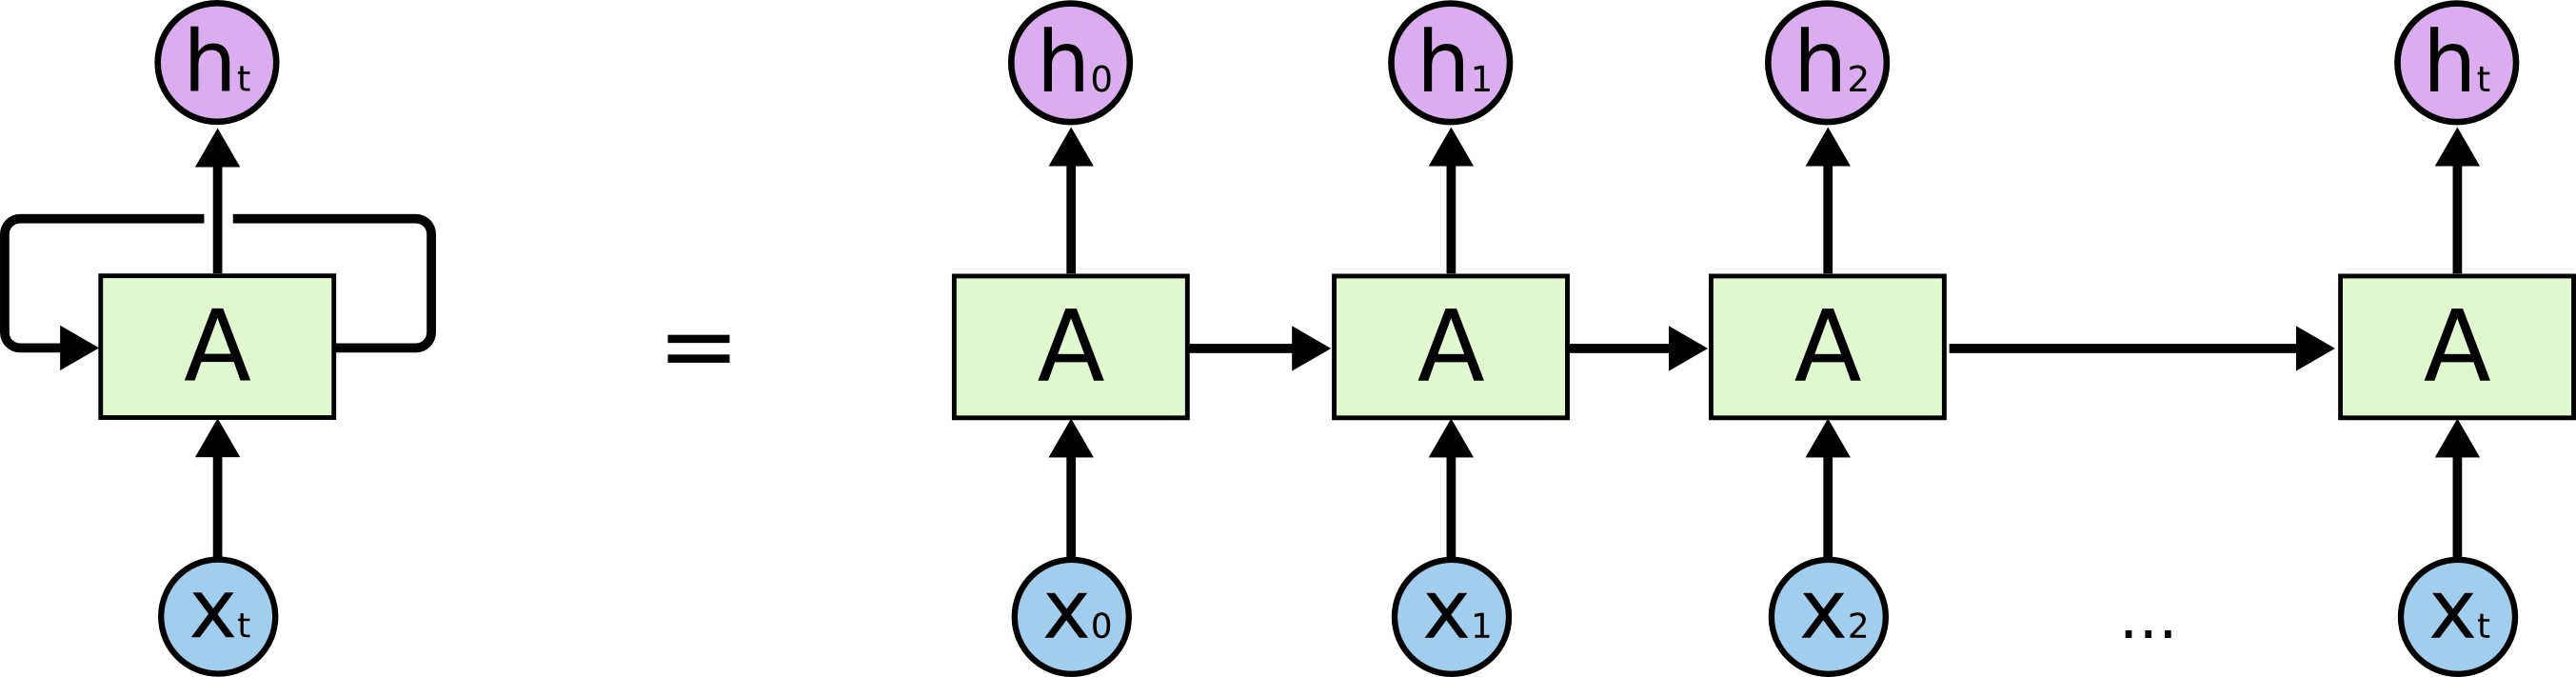
\includegraphics[width=0.80\textwidth]{RNN-unrolled}
    \caption{A graphical representation of an RNN, the left picture showing it as a loop going through a single network, and the right showing it as a sequence of identical networks. Image source: \url{http://colah.github.io/posts/2015-08-Understanding-LSTMs/}}    
    \label{fig:rnn}
\end{figure}

The number of units in the chain is equal to the number of words in the input sequence. Each unit takes in one vector representing one input word and a state vector. Each unit updates the state vector and passes it on to the next unit in the RNN chain. It also outputs a V-dimensional vector, where V is the size of the vocabulary, estimating the probability (score) that a given word follows after the current word in the input sequence. This provides a language model that can predict the next word given a word sequence. See \cite{LSTM} for a more detailed description of LSTMs.

\subsubsection{Latent Dirichlet Allocation (LDA)}

Latent Dirichlet Allocation (LDA)\cite{blei2003latent} is a generative model for text corpora that assumes each document in a corpus is generated by sampling words from a mixture of topics. The model is best described by is graphical model, seen in Figure~\ref{fig:lda}. 

\begin{figure}[htbp]
    \centering
    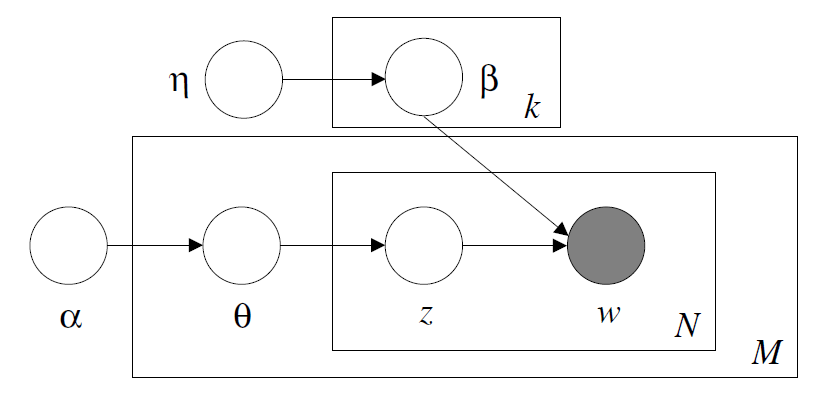
\includegraphics[width=0.70\textwidth]{lda}
    \caption{The graphical model representation of (smoothed) LDA. $w$ represents a single word in the corpus. $\alpha$ and $\eta$ are tuning parameters, $\theta$ is the mixture of topics for each document, $z$ is the topic assignment for each word in each document, and $\beta$ is the distribution of words in each topic. Image source: \cite{blei2003latent}}    
    \label{fig:lda}
\end{figure}

In LDA, each instance of a word has its own assigned topic, meaning the same word can belong to several different topics. It also means each document belongs to different topics to different extents. The topics themselves are unobserved, which means they do not need to be known or defined by someone with knowledge of the dataset, but are rather found from the data itself.

After the distributions have been learned from the data, they can among other things be used to calculate the similarity between any two documents. Seeing the topic mixture of a document as a representation of that document, a similarity measure can be calculated as the euclidean distance between two mixture vectors. This is useful for both clustering and classification of documents.

\section{Previous Work}
Perhaps the most common use of this technology is within the realm of journalism. It is clearly the domain where the average person encounters it most often as many stories nowadays are by varying degrees already written by a computer. Interestingly researchers have found that in some cases there are no significant differences in how generated text and text written by a human is perceived by the reader\autocite{RobotJournalist}. This is obviously mostly true for genuinely objective news articles and not so much for op-ed style content. In this case an algorithm could theoretically even do a better job than a human as a computer by definition has no underlying bias and has a clear speed advantage which is essential for live reporting on events such as sports or terrorist attacks.

Another interesting use case which has improved dramatically in the last few years is text summarizing. Companies such as Apple and Smmry use this to try to help the end user to ``provide an efficient manner of understanding long text by reducing it to only the most important sentences''\autocite{Smmry}. In the case of Smmry this is achieved by an algorithm that picks out the N most important sentences and displays them in the order they appeared in the original text. The end result is usually surprisingly accurate even on fairly advanced texts.

The latter of these two use cases is often used in conjunction with the former to try to differentiate from other outlets when using text written by a wholesale news agency such as the global Reuters or the Swedish TT (Tidningarns Telegrambyrå). It is also not uncommon to have an algorithm generate the story and then have a journalist revise and improve it before publishing the piece, thus capitalizing on the advantages of both technology and "the human touch"\autocite{RobotJournalist}.

\section{Method}\label{sec:method}

\subsection{Dataset}

For this project, user created content from the community of Reddit.com, the 9th most visited website in America and 30th in the world\autocite{alexa}, was used to get a good sample of interesting human written stories.

Reddit has many categories, or areas of interest, that are called ``subreddits''. We initially identified the subreddit ``Today I Fucked Up'' (\url{https://www.reddit.com/r/tifu}) as an ideal initial source of data as it contains short and humorous stories written by humans in a somewhat casual language. This subreddit has over 6 million subscribers and describes itself as \begin{quote}
A community for the dumbass in all of us. We all have those moments where we do something ridiculously stupid. Share your stories and laugh along with the internet\autocite{tifu}.
\end{quote} We also tried the following subreddits which have a strong focus on humor and personal storytelling:
\begin{itemize}
  \item Tales from Tech Support
  \item Tales from Retail
  \item Pro Revenge
  \item Petty Revenge
\end{itemize}

Reddit makes it easy to download their data via their API\autocite{redditAPI}. Using a crawler, we downloaded about 1000 posts from each subreddit, starting with the top scoring ones, to end up with a selection of high quality stories where the relative quality level was judged by the community.
The downloaded data contained the stories in addition to metadata such as title, author, views and number of comments, however only the posted texts ended up being used.

\subsection{Creating our story}
The story creation was done in several steps. First, the data was pre-processed using LDA, cleaning, and tokenization. Then the probability of word combinations were calculated using n-grams and LSTM. Finally we created new texts by sampling from the probability distributions. A more detailed description of each step follows.

\subsubsection{LDA}
To further ensure similar topics in the indata, we used LDA to cluster our documents. We opted to model 25 different topics, as we expected that should be enough to model our data while not taking too long to converge. During learning, we made use of Markov chain Monte Carlo and Gibbs sampling, as described by T. Griffiths\cite{griffiths2002gibbs}.

We approximated the mixture of topics for each document, and used the euclidean distances between the resulting vectors to calculate the similarity between different documents. We then created new, smaller datasets by selecting a random document and forming a new set from its N closest neighbours, in our case using N=200.

Using smaller datasets reduced the vocabulary to only about 20\% of the original size, which means there was a loss of variation. However, this constraint could possibly give a better coherence in the texts. 

\subsubsection{Text Processing}
The dataset of Reddit posts was pre-processed before being used to make n-grams
and train the LSTMs. In this pre-processing step we cleaned and tokenized the
raw text. Tokenization refers to the process of splitting the text into
meaningful elements, in our case words, called tokens before further processing. 
The cleaning step consisted of removing unwanted characters
like semicolons, underscores and different types of citation marks.
We also removed all characters marking the end of a sentence like periods,
question marks and exclamation marks and replaced these characters with
$<eos>$. This was done in order to model the ending of sentences more easily.
The tasks of marking the end of sentences and tokenize the raw text were made 
easy due to functionality provided by the Python library NLTK \cite{NLTK}.

\subsubsection{n-grams}
A discussion of N-gram order by Russell and Norvig\autocite{AiModernApproach} demonstrates that unigrams are a poor representation of the English language and that bigrams and trigrams provide better approximations. Unigrams perform poorly due to the loss of any ordering based on previous words or tokens. For this reason we constructed several different n-gram models, from 5- to 2-grams, and queried them in order from largest to smallest until a sufficiently large selections of predictions, along with their probabilities, had been obtained. These were normalized and joined together in a manner that ensured words suggested by larger n-grams models had a higher probability than those suggested by smaller n-grams.

When constructing the n-grams the training text was considered as one long sequence where sentence ends were replaced by end-of-sentence marker \texttt{<eos>}. This resulted in n-grams where the \texttt{<eos>} marker could appear at any position and was done in order to effect the possibility of some continuity from one sentence to anther during text generation.

\subsubsection{LSTM}\label{sec:methodlstm}
Our n-gram scores were combined with scores from LSTM models. We based our LSTM solution on the LSTM small, non-regularized network architecture presented in \cite{Zaremba14}. We have trained this network first on the Penn Tree Bank (PTB) English news dataset \cite{PTB} and then also on our preprocessed input texts from reddit, finally having one LSTM model for each subreddit. The training was done in TensorFlow, see \cite{TensorFlow} for more details on the training procedure. All words unknown to the word embeddings were replaced with the $<unk>$ token both when training and when evaluating the model. This enabled us to always use the same network architecture with the same output dimension (10000 words in our case).

When generating stories, the LSTM was evaluated on up to 30 words (a tunable parameter) of the preceding output text sequence. 

\subsubsection{Score Combination and Next Word Sampling}
The scores of the n-grams and the LSTM were then combined. First, we had to ensure that all the scores were non-negative. All negative LSTM scores were replaced with zeros. The n-gram model suggested a set of at least 10 possible story continuing words and their probabilities. The combined n-gram score for a word w out of this set
\begin{equation}
s_{ng,w}= d^{n-2} s_{n,w}
\end{equation}
was obtained from the highest n-gram model (index n) mentioning the word w, where $s_{n,w}$ is the score of the highest n-gram model and d is a tunable decay parameter. We used $d=3$. The lowest possible n-gram (bigram) had $n=2$.

After normalizing both the combined n-gram and LSTM score ($s_{l,w}$) vectors to sum to one, we performed an element-wise multiplication of these two normalized (probability) vectors.
\begin{equation}
s_{c,w}= \frac{s_{ng,w} s_{l,w}}{\sum_w{s_{ng,w}} \sum_w{s_{l,w}}}
\end{equation}
This combined score $s_{c,w}$ was then again normalized to sum to one and became our final probability distribution. We sampled a word to append to the story from this distribution by utilizing functions of the NLTK library \cite{NLTK}.

A sentence could end in 2 possible ways:
\begin{enumerate}
\item With probability 50\% (tunable) if the LSTM gave the highest score to the sentence terminator token, $<eos>$.
\item With probability proportional to $0.02 \times \max_w{s_{ng,w}} \times s_{l,w}$ (normalized).
\end{enumerate}

\subsection{Presentation}
The generated stories were presented in a user friendly manner by creating a website alongside the full source code on GitHub (\url{http://powion.github.io/storybot/}). Here the user can select from the different subreddits described in Section~\ref{sec:method} and get a selection of generated stories for that theme.

\section{Results}
The first results we got were from a method using only n-grams. Already you could see the essence of the subreddit in the text, for example text generated from Today I Fucked Up clearly mentioned problematic situations. The overall grammar and consistency was not perfect however, and a big problem was that the sentences got very long and rambling. An example is this sentence generated from the Today I Fucked Up data:
\begin{quotation}
"Today I was so horny that I disregarded the fact of what a stupid idea, but when you really think about it, step to the alley and throw up bacardi 151, then crash through the doors and yell ``where the fuck did that come from?!'' yeah."
\end{quotation}
The next step was adding LSTMs. This improved grammar slightly since they were trained on news and not just reddit posts. Furthermore, the LSTMs favored much shorter sentences, to the point where we had to artificially lower the probability of selecting a sentence terminator, as described in Section~\ref{sec:methodlstm}. Below is an example of a text generated from Tales from Tech Support. 
\begin{quotation}
"Never heard of such a thing. What person needs \$ 1200 of credit the only catch was getting business cards from his house. I went out and got another job and just decided to cut the coax. And was told that the only port for this on his laptop. I think back to the last couple of times I was holding. I got up from my chair staring at me. The user made an excuse. I tried to think of it. I've never used that. The head builder started smiling."
\end{quotation}
While the text fragments here are from at least 25 different parts of the corpus, there is still some persistent theme in the text. The general feel is similar to that of the posts in the original subreddit. 

The LDA topic models were tried after after this. When examining the most common words for each topic in our models, it was hard to see any patterns at first. However, each subreddit gave at least a few topics that showed some coherence. Following are the top 10 words of select topics from Petty Revenge and Today I Fucked Up respectively.
\begin{quotation}
heavily, bankers, hyperexcited, mastiff, violating, scratching, terrier, owed, howls, homemade
\end{quotation}
\begin{quotation}
squirming, nvidia, overnight, corners, gaming, wee, packets, hormones, foliageheavy, reesez
\end{quotation}
Following is an example from Tales from Tech Support, generated from a 200-post cluster:
\begin{quotation}
This lady's response was completely different from the rest not even the power light. Customer : no I ca christmas. User : no. It is easy right so what is the problem myself. Me : you know exactly what you didn't do much. You put serious experience ended drinking decision. I took back internet explorer. I'll just install chrome. Poor situation. I call back a few minutes later.
\end{quotation}
In the end, we did not see any great improvements when using the clustered data compared to using the full dataset.

\section{Conclusions and Discussion}
The quality of the stories depended on the quality of the dataset. This was of course the point of the project, but it also introduced some difficulties. Since Reddit posts are often not fully grammatically correct, the grammar in our stories is not perfect. Also, this discrepancy from correct grammar made it more difficult to use other datasets such as news articles for additional grammar data. 

Our algorithms generated stories only by looking into the past text output. Exploring the storyline into the future or adding semantic models could further improve the output quality.

Regarding the LDA models, it is possible that there were not really any larger distinct topics within the subreddits, since they already belong to the topic of the subreddit itself. To improve the performance for this part, we could have tried to identify the most coherent topics and rely more heavily on those for calculating similarity. We could also have used a more advanced clustering algorithm. 

\printbibliography[heading=bibnumbered]
%\bibliography{refs}{}

\end{document}
